\documentclass[a4paper]{article}

\usepackage{amsmath}
\usepackage{graphicx}
\usepackage{hyperref}
\usepackage{tabularx}

\title{Forensics analysis of USB device traces\\
\large Digital Forensics}

\author{
\begin{tabular}{>{\raggedleft}m{5cm}m{5cm}}
I. Duits & (1876171) \\
E. Geretto & (1869426) \\
G. Iadarola & (1879480) \\
\end{tabular}
}

\begin{document}
\maketitle

\section{Introduction}
Nowadays, almost half of all households in Western Europe have a personal
computer and the percentage increases over 90\% by taking into account only
young people (15 to 30 years old).

The number of computing devices as PCs, laptops and smartphones has increased
exponentially in the past decade. Daily activities are organized on social
media, works are performed on laptop and meetings on video-conference. Our
entire life is managed through electronic devices and the number of connected
user is going to grow in the future. The government's (most of them) and the
public opinion do agree with these changes and support every initiative which
increase the use of new technologies.

Nevertheless, several problems has to be faced and need to be managed in order
to keep benefiting from the computing devices revolution.

Everyone can get access and interact with PCs and smartphones and also criminals
are using them to perpetrate frauds and illegal activities. Indeed, the Digital
forensic branch is becoming one of the most important sector in the forensics
and investigation field. By inspecting and analysing computer systems, officers
can retrieve essential evidence to prove and demonstrate criminal event.

This paper aims to contribute in this field and is focused on USB devices and
the traces left on operating systems.

USB devices can be used to transfer valuable data in cases of data theft or
possession of illegal material, and knowledge about when a USB device was
connected can be really helpful in the investigation.

As stated in the Locard's exchange principle~\cite{locard2008locard}, copying
data leaves traces. These traces are recoverable as reported for instance by
several researches available in the literature.~\cite{Tanushree12,Abhijeet14}.

In Section~\ref{sec:lit} is discussed how to access this information in both
Windows and Linux systems. On windows environment, there are many tools which
can help us in analysing and retrieving data. However, on Linux there are just
few useful tools.

Windows is the most used operating systems but Linux usage is
increasing~\cite{osShare} and actually most of the servers run on a Linux
distribution~\cite{InternetServer}. In order to contribute in the digital
forensic field on Linux systems, a tool was developed by us and subsequently
opensourced. This software will help Linux users in retrieving data about USB
devices from an image of Linux installation.

The paper is structured as follow. In section~\ref{sec:resprep} is described the
methodology and the steps performed to analyse the images which were used to
develop the tool. Then, the achieved goals are described in
section~\ref{sec:goals} and the short discussion reported in
section~\ref{sec:concl} ends the paper.

\section{Literature}\label{sec:lit}
The log files on a computer distribution can be used to track the use of usb
devices on the system.  Log files records the history of events and executions
in detail, which can be used to see the earlier or current state of a system and
to recover such a state \cite{logFiles}. They can be also used to detect
unexpected behavior and track suspicious activities that may violate the system,
this is useful for both private users and digital forensics.

\subsection{Windows}\label{sec:litWindows}
Windows 8 and 10 have a program installed, Event Viewer, which allows users to
view the log and look up all the information. The tool can be used to track down
the usages of usb sticks. For a detailed explanation on how to use it, go to
\cite{eventViewerW10}. For this tool the computer needs to be running.

In digital forensics it is not always possible to just boot the computer and
look for the log file, that will make changes to the system. An image of the
computer is therefore created, which can be investigated instead.

There are different kind of software tools which can help to search the log
files of an image, and thus the connection of usb devices on a Windows system.
For example the open source tool Autopsy\footnote{\url{http://www.autopsy.com/}}
can be used to read the image and extract all kind of useful information from
it. The connection time and usb serial number can be found really easily.

\subsection{Linux}
Less information can be found on how to obtain usb device tracking information
on a Linux system. For example, figure \ref{fig:linuxlog}
\cite{USBdeviceTracking} shows where to find the log file, and which information
the file holds.
\begin{figure}[h]
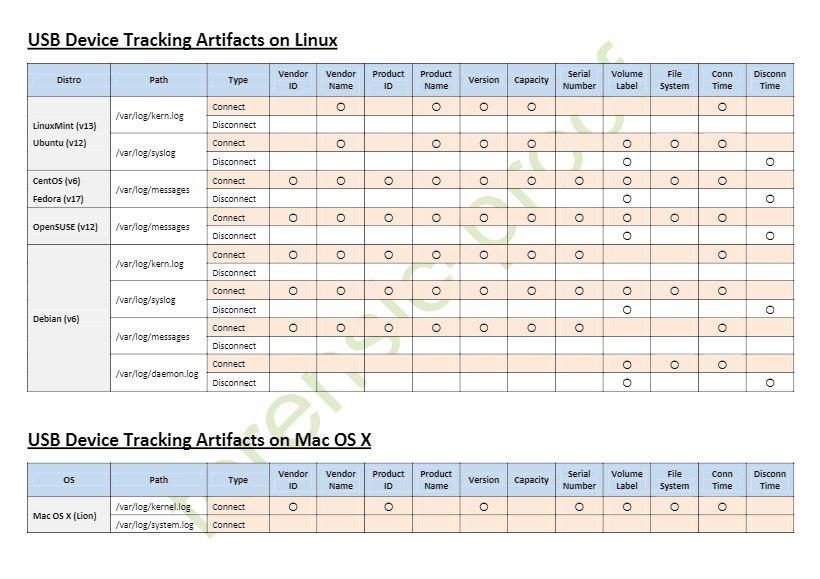
\includegraphics[width=\linewidth]{linux.jpg}
\label{fig:linuxlog}
\end{figure}
Unfortunately the information is way outdated. This file was published in 2012
and the paths to the log files is incorrect.




\section{The research preparation}
\label{sec:resprep}
\subsection{General plan}
For this research we will create a few images of different Linux distributions,
which ones will be discussed in section \ref{sec:usedLinux} and how we create
them is discussed in section \ref{sec:createImage}. We will then analyze the
created images' log files by a python program we wrote, which is explained in
section \ref{sec:python}

\subsection{Used Linux distribution systems}\label{sec:usedLinux}
We are using the following Linux distributions.
\begin{itemize}
\item Fedora 25, kernel 4.8.6
\item OpenSUSE
\item Ubuntu
\item Debian
\end{itemize}
For each Linux we used the last stable version, we start installing the
distributions on May 29 2017. With these distributions mentioned above, we cover
most of the popular Linux distro's \cite{LinuxDistro}, as we can see that some
other Linux distro's are part of these. Distributions like Elementary, Linux
Mint and  Zorin are all Ubuntu based and thus covered in our research. % other
website with top10 distro
https://brashear.me/blog/2015/08/24/results-of-the-2015-slash-r-slash-linux-distribution-survey/

\subsection{Creating the images}\label{sec:createImage}
The following steps were taken to prepare for the research:
\begin{itemize}
\item Clear the computer
\item Install the Linux Distribution (default installation, version as mentioned in Section \ref{sec:usedLinux})
\subitem Make sure all drives work correctly (Note: this influence the log file)
\item Then we repeat 5 times, the following sequence
\subitem Start up
\subitem Plug in mouse
\subitem Plug in USB 2.0
\subitem Plug in USB 3.0
\item Create image of the machine
\end{itemize}

\subsection{The program in Python}\label{sec:python}


\section{Found results}
\label{sec:goals}


\section{Conclusion}
\label{sec:concl}



Analyzing the log fies of a system could besides tracking usb usages, be very
useful for other digital forensic applications, like finding unexpected behavior
and track the use of the computer.


\bibliographystyle{abbrv}
\bibliography{sample}

\end{document}
